\section{Carat Data}

The Carat data consists of samples containing mobile device system settings, current battery level, the list of currently running mobile applications and a user specific identification token unique to each Carat application installation. Each Carat application user periodically sends these samples to the Carat server, typically when the device's battery level changes~\cite{Oliner:2013:CCE:2517351.2517354}. 

Since we are interested about the effects that the mobile devices system settings and state may have on the energy consumption rate of the device, the samples need to be converted in such a way that the energy rate becomes accessible. This was done by grouping all samples according to their user identification token. The grouped tokens were then sorted according to the time of the samples arrival time stamp. These sorted samples were then paired up so that the first sample and the second sample make up pair number 1, the second and the third sample make up sample pair number 2 and so forth. These sample pairs were used as the basis of this analysis. The energy rate of a sample pair was calculated as the difference of the samples' battery levels divided by the difference of their time stamps. The set of running applications for a sample pair was decided to be the union of both samples running applications. For all other system settings and state the more recent of the sample pairs was used to determine the state or setting of the sample pair.

Since the Carat data comes from a large number of unsupervised clients, there is no guarantee for the integrity of the data. A faulty device or a hostile client may produce erroneous data. It is therefore essential to apply filtering to the data to minimize the amount errors in the data. 

Let us give a brief description of each of the system settings and state variables that were used as part of the analysis. Association analysis requires discrete data, as explained in chapter~\ref{association analysis}. Therefore we describe the way each of these variables is discretized. The following presentation of the data is based on a subset of the Carat data consisting of samples that were collected between 26.8.2016 and 3.10.2016 that had Facebook mobile application running.

\subsection{Energy Rate}

Energy rate of a mobile device is the velocity at which the mobile devices battery is discharging. The unit of the energy rate is percentage per second. This means that an energy rate of $\frac{0.05}{s}$ would drain the whole battery in just $\frac{100}{0.05 / s} = 2000 s \approx 33 minutes$.

\begin{figure}[!htbp]
	\centering
	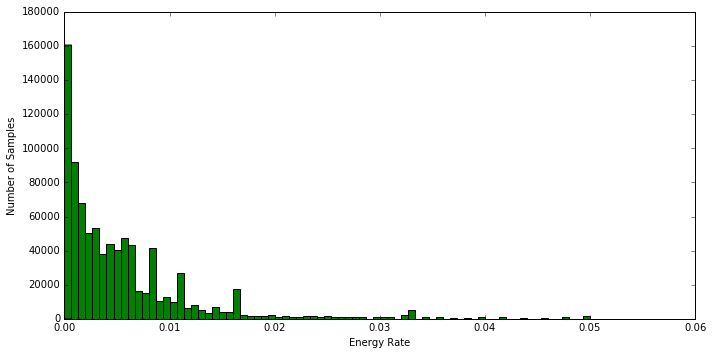
\includegraphics[width=\textwidth]{images/carat-data/energy_rate.png}
	\caption{Histogram of energy rates with 75 bins}
	\label{figure:carat-data-energy-rate}
\end{figure}  

Figure~\ref{figure:carat-data-energy-rate} shows a histogram of the energy rate distribution. The distribution seems to be a rough approximation of an exponential distribution. The distribution does not seem have an evident categorical division. Thus, the data was discretized by dividing it to four bins of equal frequency. 

\subsection{CPU Usage Level}  

CPU usage level is the fraction of time that the central processing unit(s) of the mobile device were busy when the sample was collected. The CPU usage level is in a unit of percentages of the maximum level. All CPU usage levels that were below zero or greater than 100 were discarded as faulty data.

\begin{figure}[!htbp]
	\centering
	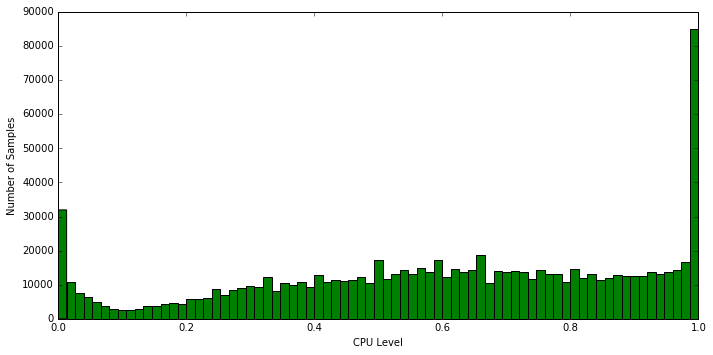
\includegraphics[width=\textwidth]{images/carat-data/cpu_level.png}
	\caption{Histogram of CPU usage levels with 75 bins}
	\label{figure:carat-data-cpu-level}
\end{figure}  

Figure~\ref{figure:carat-data-cpu-level} shows a histogram of the CPU usage level distribution. The distribution very roughly approximates the uniform distribution except for 100\% and 0\% CPU usage levels, which are quite overrepresented. The data was discretized into four bins of equal frequency.

\subsection{Travel Distance}  

Travel distance is the distance in meters, that the mobile device moved between the two samples. 

\begin{figure}[!htbp]
	\centering
	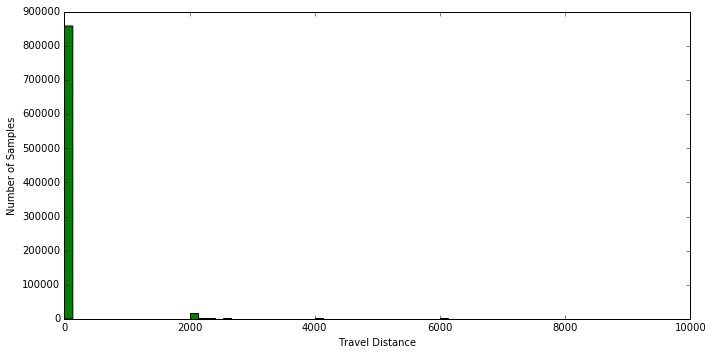
\includegraphics[width=\textwidth]{images/carat-data/travel_distance.png}
	\caption{Histogram of travel distance with 75 bins}
	\label{figure:carat-data-travel-distance}
\end{figure}  

Figure~\ref{figure:carat-data-travel-distance} shows a histogram of the travel distance distribution. Most of the mass of the distribution is concentrated in the close proximity of zero with other values having very low frequencies. The travel distance was discretized to two categories: \textit{moving}, if the travelled distance was greater than 100 meters, and \textit{static} otherwise.

\subsection{Battery Temperature}  

Battery temperature is the measured mobile device battery temperature in degrees Celsius. Temperatures smaller than five degrees were discarded as it is very rare for a battery temperature to be that low even in subzero climates. Likewise battery temperatures of over 100 degrees were discarded, as healthy devices very rarely reach such high battery temperatures.

\begin{figure}[!htbp]
	\centering
	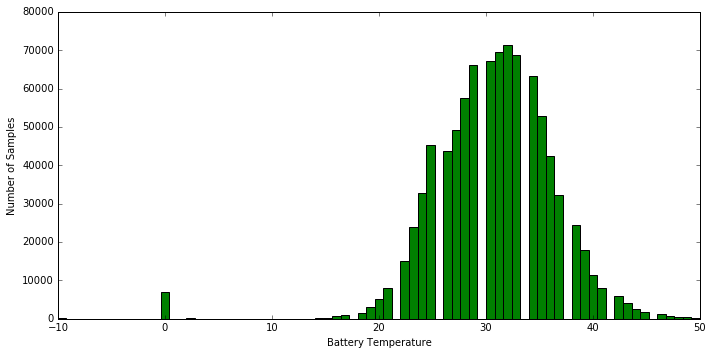
\includegraphics[width=\textwidth]{images/carat-data/battery_temperature.png}
	\caption{Histogram of battery temperatures with 75 bins}
	\label{figure:carat-data-battery-temperature}
\end{figure}  

Figure~\ref{figure:carat-data-battery-temperature} shows a histogram of the battery temperature distribution. The distribution approximates a normal distribution with some skewedness. There is also a small cluster of measurements near zero degrees Celsius. This is most likely due to mobile devices systematically reporting a value of zero if the measurement data is not available. The data was discretized into four bins of equal frequency.

\subsection{Battery Voltage}  

\subsection{Screen Brightness}  

\subsection{Mobile Network Technology}  

\subsection{Network Type}  

\subsection{WiFi Signal Strength}

\subsection{WiFi Connection Speed}  